\section*{Exercise Part (A) - The 7-stage RISC Pipeline}

\begin{enumerate}[wide, label=(A\arabic*)]

% (A1) How many stalls (clock-cycles) occur, on LOAD instructions (when the instruction following a LOAD instruction uses the value being loaded) ? Use an excell timing diagram to illustrate your answer, and use an arrow (or asterisks *) to illustrate when data is FORWARDED. (Please see the class notes - the timing diagram has instructions along the y-axis, and clock-cycles along the x-axis. A sample excel file is posted on Avenue-to-Learn.) • Add a comment for every forwarding of data or signals that occurs. A comment might be ‘*forward R0 (EX* to *D) in cc 7’.
\item 
There is a 2 clock-cycle stall on LOAD instructions when the instruction following a LOAD instruction uses the value being loaded. The timing diagram can be seen in Figure~\ref{fig:A1}.

% How many branch-delay-slots (clock-cycles) occur, following a BRANCH instruction?
% Make the same assumptions as in the class notes: Consider an instruction BNEZ R0, loop. Assume that branches are resolved as soon as possible, in the ID stage, without “stretching the clock”. This leads to 2 cases to consider, as described in the class notes:
\item
The number of branch-delay-slots following a BRANCH instruction will depend on the case considered:
\begin{enumerate}[wide, label=\arabic*.]
% (1) If the value R0 being tested is available in a register at the start of the ID stage, then the “branch is resolved” in the ID stage - the ID stage will compare R0 with zero, and generate a “Take-Branch” signal which is sent back to the IF1 stage from the ID stage in clock-cycle 3. (See class notes in 4DM4 Lecture 10.)
\item If the value R0 being tested is available in a register at the start of the ID stage, then the “branch is resolved” in the ID stage - the ID stage will compare R0 with zero, and generate a “Take-Branch” signal which is sent back to the IF1 stage from the ID stage in clock-cycle 3. In this case, 2 branch-delay-slots will occur, as seen in Figure~\ref{fig:A2.1}. The compiler can attempt to fill the "BRANCH+1" and "BRANCH+2" branch delay slots with useful instructions, otherwise fill with a NO-OP. 

% If the value R0 is being computed in the EX stage, by the previous instruction, and R0 needs to be forwarded to the ID stage, then we do not “stretch the clock” to allow R0 to be tested in the ID stage in the same clock cycle. The system will “stall” the BNEZ for 1 extra clock cycle, waiting for R0 to be computed and forwarded to the ID stage. (See class notes in 4DM4 Lecture 13a, Tutorial #4.)
\item If the value R0 is being computed in the EX stage, by the previous instruction, and R0 needs to be forwarded to the ID stage, then we do not “stretch the clock” to allow R0 to be tested in the ID stage in the same clock cycle. The system will “stall” the BNEZ for 1 extra clock cycle, waiting for R0 to be computed and forwarded to the ID stage. In this case, 2 branch-delay-slots will occur, as seen in Figure~\ref{fig:A2.2}. The compiler can attempt to fill the "BRANCH+1" and "BRANCH+2" branch delay slots with useful instructions, otherwise fill with a NO-OP.
\end{enumerate}
\end{enumerate}

\begin{figure}[htp]
    \centering
    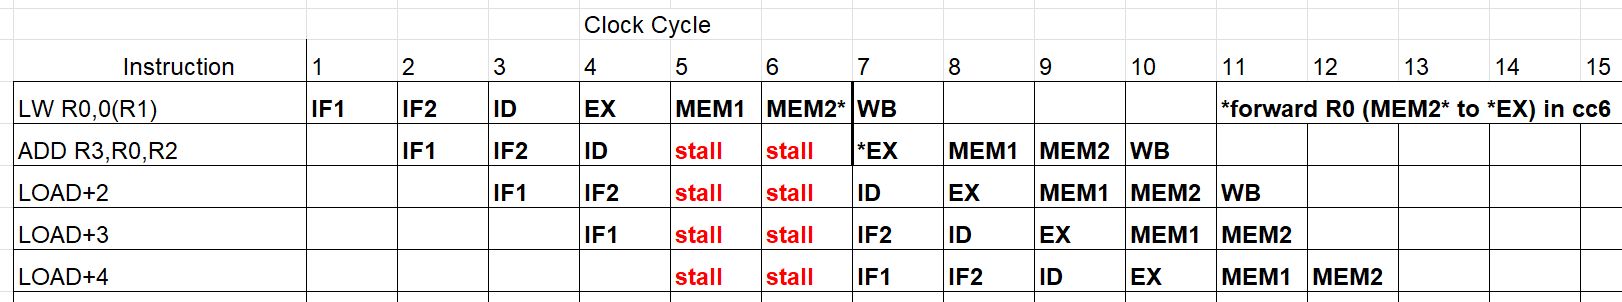
\includegraphics[width=0.85\textwidth]{a1.png}
    \caption{\label{fig:A1}Timing Diagram for A1}
\end{figure}

\begin{figure}[htp]
    \centering
    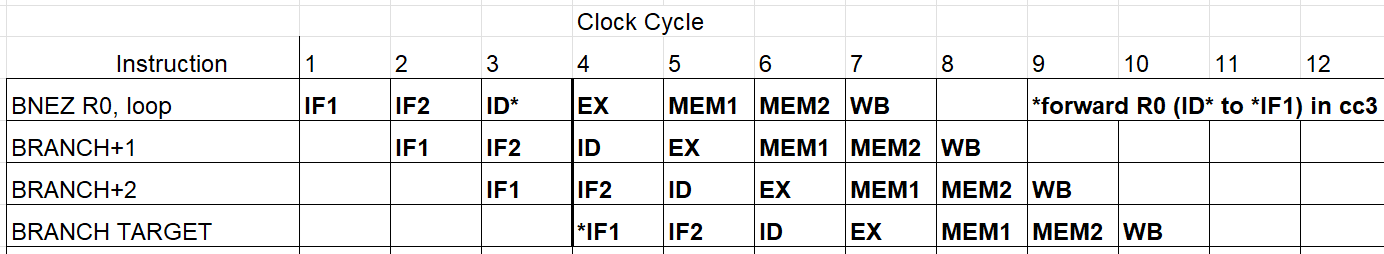
\includegraphics[width=0.85\textwidth]{a2.1.png}
    \caption{\label{fig:A2.1}Timing Diagram for A2 Case 1}
\end{figure}

\begin{figure}[htp]
    \centering
    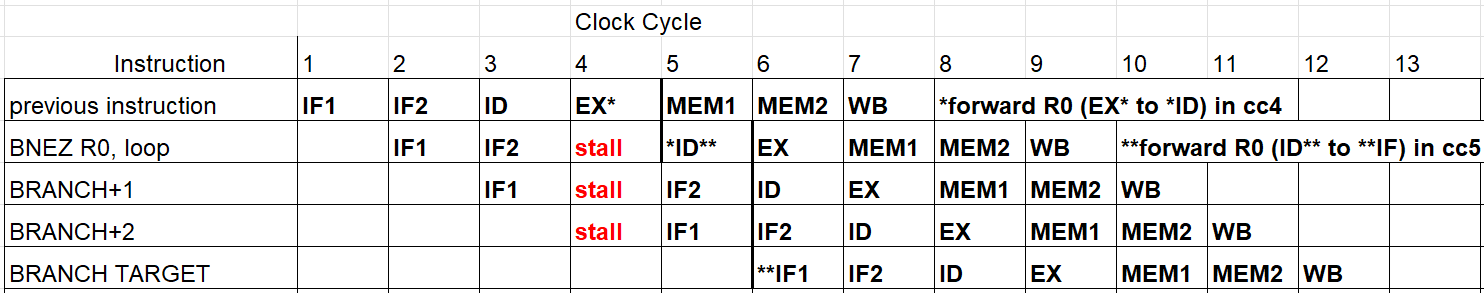
\includegraphics[width=0.85\textwidth]{a2.2.png}
    \caption{\label{fig:A2.2}Timing Diagram for A2 Case 2}
\end{figure}